\documentclass{article}
\usepackage[utf8]{inputenc}
\usepackage{fullpage}
\usepackage{amsmath}
\usepackage{graphicx}
\graphicspath{ {./images/} }

\title{Feynman's Technique for Computing Integrals}
\author{Tyler Lin}

\begin{document}

\maketitle

\section*{Introduction}
During his high school years, renowned American theoretical physicist Richard Feynman was not the best student. Though clearly gifted, he struggled to stay engaged in class. One day, Feynman's physics teacher, Mr. Bader, pulled Feynman after class and said to him, 
\begin{quote}
    “Feynman, you talk too much and you make too much noise. I know why. You’re bored. So I’m going to give you a book. You go up there in the back, in the corner, and study this book, and when you know everything that’s in this book, you can talk again” (Feynman).
\end{quote}
The book was \textit{Advanced Calculus}, published in 1926 by MIT mathematician Frederick S. Woods. It contained all kinds of concepts that Feynman didn't know about, including a method of solving integrals called the \textbf{Leibniz Integral Rule}. The Leibniz Integral Rule, also known as differentiation under the integral time, is not emphasized in university, but Feynman would use it time and time again. 
\newline \newline According to Feynman, 
\begin{quote}
    "when guys at MIT or Princeton had trouble doing a certain integral, it was because they couldn’t do it with the standard methods they had learned in school...Then I come along and try differentiating under the integral sign, and often it worked. So I got a great reputation for doing integrals, only because my box of tools was different from everybody else’s."
\end{quote}
This article is about the Leibniz Integral rule, which is colloquially referred to as \textbf{Feynman's Technique for Computing Integrals}.
\subsection*{How Feynman's Technique Works}
Leibniz's Rule states that given a differentiable function $f(x,k)$,
$$\frac{d}{dk}\bigg(\int_{a}^{b}f(x,k)dx\bigg)=\int_{a}^{b}\frac{\partial}{\partial k}f(x,k)dx.$$
In other words, it is possible to interchange the derivative operator and the integral in certain circumstances. Feynman's Technique employs this rule to change a seemingly impossible integral into a solvable differential equation.
\section*{Examples}
\subsection*{Problem 1}
Evaluate $$\int_{0}^{1}\frac{x^2-1}{\ln{x}}dx.$$
The integrand must have two unknowns to apply Feynman's technique, so we introduce the constant $k$ such that
\begin{equation}
    g(k) = \int_{0}^{1}\frac{x^k-1}{\ln{x}}dx
\end{equation} for $k>0$. This step (assigning a new variable) is the most difficult part, and in some cases there won't be any suitable options. Fortunately, in this case, replacing the exponent with $k$ will later allow us to cancel out the $\ln(x).$
\newline We proceed with \textbf{differentiating under the integral sign}.
\begin{equation*}
    \begin{split}
        \frac{dg}{dk} &= \frac{d}{dk}\int_{0}^{1}\frac{x^k-1}{\ln{x}}dx \\
        &= \int_{0}^{1}\frac{\partial}{\partial k}\frac{x^k-1}{\ln{x}}dx \\
        &= \int_{0}^{1}\frac{x^k\ln{x}}{\ln{x}}dx \\
        &= \int_{0}^{1}x^kdx \\
        &= \frac{x^{k+1}}{k+1}\bigg\vert_{0}^{1} \\
        &= \frac{1}{k+1}.
    \end{split}
\end{equation*}
Therefore $$g(k)=\ln{|k+1|}+C.$$
As our final step, we must find $C$ using our original equation $$g(k) = \int_{0}^{1}\frac{x^k-1}{\ln{x}}dx.$$ Logically, we start with $k=0$. 
$$g(0)=\int_{0}^{1}\frac{1-1}{\ln{x}}dx = 0.$$
Substituting into equation 1,
\begin{equation*}
    \begin{split}
        g(0) &= \ln{|0+1|}+C \\
        0 &= 0+C \\
        C &= 0 \\
        g(k) &= \ln{|k+1|}.
    \end{split}
\end{equation*}
Finally, to solve the original integral we calculate $g(2)$.
$$\int_{0}^{1}\frac{x^2-1}{\ln{x}}dx = g(2) = \boxed{\ln({3})}.$$
Not bad! Here is a more complicated example.
\subsection*{Problem 2}
Evaluate $$\int_{0}^{\pi} \ln(1-2\alpha\cos{x}+\alpha^2)dx$$ for $|\alpha|<1$.
\newline Again, the usual tricks will not result in a solution; the reader can attempt it if they wish. It turns out that Feynman's Technique is the only method that works.
\newline This time, there are already two variables in the integrand, $\alpha$ and $x$. In this case, we will treat the integral as a function of $\alpha$.
$$f(\alpha)=\int_{0}^{\pi}\ln(1-2\alpha\cos{x}+\alpha^2)dx.$$
\newline Now we \textbf{differentiate under the integral sign} with respect to alpha.
\begin{equation*}
    \begin{split}
        \frac{df}{d\alpha} &=  \frac{d}{d\alpha}\int_{0}^{\pi}\frac{-2\cos{x}+2\alpha}{1-2\alpha\cos{x}+\alpha^2}dx \\ 
        &= \int_{0}^{\pi}\frac{\partial}{\partial \alpha}\ln(1-2\alpha\cos{x}+\alpha^2)dx \\
        &= \int_{0}^{\pi}\frac{-2\cos{x}+2\alpha}{1-2\alpha\cos{x}+\alpha^2}dx.
    \end{split}
\end{equation*}
While this looks messy, it is indeed solvable.
\begin{equation*}
    \begin{split}
        \int_{0}^{\pi}\frac{-2\cos{x}+2\alpha}{1-2\alpha\cos{x}+\alpha^2}dx &= \frac{1}{\alpha}\int_{0}^{\pi}\frac{-2\alpha\cos{x}+2\alpha^2}{1-2\alpha\cos{x}+\alpha^2}dx \\&= \frac{1}{\alpha}\int_{0}^{\pi}\frac{-2\alpha\cos{x}+2\alpha^2}{1-2\alpha\cos{x}+\alpha^2}dx - 1 + 1
        \\&=\frac{1}{\alpha}\int_{0}^{\pi}\frac{-2\alpha\cos{x}+2\alpha^2}{1-2\alpha\cos{x}+\alpha^2}dx - \frac{1-2\alpha\cos{x}+\alpha^2}{1-2\alpha\cos{x}+\alpha^2} + 1
        \\&=\frac{1}{\alpha}\int_{0}^{\pi}\frac{\alpha^2-1}{1-2\alpha\cos{x}+\alpha^2}dx + 1 \\&= \frac{1}{\alpha}\int_{0}^{\pi}1 - \frac{1-\alpha^2}{1-2\alpha\cos{x}+\alpha^2}dx.
    \end{split}
\end{equation*}
Dividing everything by $1+\alpha^2$, we get
\begin{equation}
    \begin{split}
        \frac{df}{d\alpha} &= \frac{1}{\alpha}\bigg(\pi-\frac{1-\alpha^2}{1+\alpha^2}\bigg)\int_{0}^{\pi}\frac{1}{1-\frac{2\alpha}{1+\alpha^2}\cos{x}}dx \\&= \frac{\pi}{\alpha}-\bigg(\frac{1}{\alpha}\bigg)\bigg(\frac{1-\alpha^2}{1+\alpha^2}\bigg)\int_{0}^{\pi}\frac{1}{1-\frac{2\alpha}{1+\alpha^2}\cos{x}}dx.
    \end{split}
\end{equation}
Finally, the rightmost integral is solvable! We use a reverse $u$ substitution: let $x=2\arctan{u}$. Then $\cos{x}=\frac{1-u^2}{1+u^2}$, $u=\tan{\frac{x}{2}}$, and $dx=\frac{2du}{1+u^2}$.
\begin{equation*}
    \begin{split}
        \int_{0}^{\pi}\frac{1}{1-\frac{2\alpha}{1+\alpha^2}\cos{x}}dx &= \int_{0}^{\pi}\frac{2du}{1-\frac{2\alpha}{1+\alpha^2}\frac{1-u^2}{1+u^2}}\\
        &= \int_{0}^{\pi}\frac{2du}{1+u^2-\frac{2\alpha(1-u^2)}{1+\alpha^2}} \\&= \int_{0}^{\pi}\frac{2(1+\alpha^2)du}{(1+u^2)(1+\alpha^2)-2\alpha(1-u^2)}
        \\&= \int_{0}^{\pi}\frac{2(1+\alpha^2)du}{1+u^2+\alpha^2+u^2\alpha^2-2\alpha+2\alpha u^2} \\&= \int_{0}^{\pi}\frac{2(1+\alpha^2)du}{1-2\alpha+\alpha^2+u^2(1+2\alpha+\alpha^2)}\\&= \int_{0}^{\pi}\frac{2(1+\alpha^2)du}{(1-\alpha)^2+(1+\alpha)^2u^2} \\&= \frac{2(1+\alpha^2)}{(1-\alpha)^2}\int_{0}^{\pi}\frac{du}{1+(\frac{1+\alpha}{1-\alpha})^2u^2}.
    \end{split}
\end{equation*}
Note that $\frac{1+\alpha}{1-\alpha}$ ranges from 0 to $-\infty$ because $|\alpha|<1$. To simplify things, we declare a constant $\beta$ such that $$\beta=\frac{1+\alpha}{1-\alpha}u \text{ and } d\beta=\frac{1+\alpha}{1-\alpha}du \text { (so } du=\frac{1-\alpha}{1+\alpha}d\beta \text{)}.$$
Substituting,
$$\frac{2(1+\alpha^2)}{(1-\alpha)^2}\int_{0}^{\pi}\frac{du}{1+(\frac{1+\alpha}{1-\alpha})^2u^2} = \frac{2(1+\alpha^2)}{(1-\alpha)(1+\alpha)}\int_{0}^{-\infty}\frac{d\beta}{1+\beta^2}.$$
This looks familiar, it's arctan!
\begin{equation*}
    \begin{split}
        \frac{2(1+\alpha^2)}{(1-\alpha)(1+\alpha)}\int_{0}^{-\infty}\frac{d\beta}{1+\beta^2} &= \frac{2(1+\alpha^2)}{1-\alpha^2}\arctan{\beta}\bigg\vert_{0}^{-\infty}
        \\&= \frac{2(1+\alpha^2)}{1-\alpha^2}(\frac{-\pi}{2}) \\&= \frac{-\pi(1+\alpha^2)}{1-\alpha^2}.
    \end{split}
\end{equation*}
The integral portion of equation 2 is now simplified, but we must not forget the multipliers.
$$\frac{df}{d\alpha} = \frac{\pi}{\alpha}-\bigg(\frac{1}{\alpha}\bigg)\bigg(\frac{1-\alpha^2}{1+\alpha^2}\bigg)\frac{-\pi(1+\alpha^2)}{1-\alpha^2} = \frac{\pi}{\alpha}-\frac{-\pi}{\alpha} = \frac{2\pi}{\alpha}.$$
We can now solve for $f(\alpha)$ by integrating:
\begin{equation}
    f(\alpha) = 2\pi\ln{|\alpha|}+C.
\end{equation}
Our final step is to find $C$ using our original equation,
$$f(\alpha)=\int_{0}^{\pi}\ln(1-2\alpha\cos{x}+\alpha^2)dx.$$
We first consider substituting $\alpha=0$, but we note that it would give us $\ln{(0)}$ in equation 3, which is undefined. We try $\alpha=1$ next:
$$f(1)=\int_{0}^{\pi} \ln(2-2\cos{x})dx.$$
This integral evaluates to 0. The derivation is left as a exercise to the reader.
\newline It follows that
$$f(1)=2\pi\ln{(1)}+C=0+C=0,$$ so $C=0.$
Finishing up,
$$\int_{0}^{\pi} \ln(1-2\alpha\cos{x}+\alpha^2)dx \text{ for } |\alpha|<1 = f(\alpha) = \boxed{2\pi\ln{|\alpha|}}.$$ 
The technique of differentiating under the integral sign is not commonly used, but very powerful in certain situations.

\section*{Exercises for the Reader}
The solution to these integrals are much shorter than the first example, so don't hesitate to try them.
\newline \newline 1. Use Feynman's technique to evaluate
$$\int_{0}^{1}(2x+k^3)^2dx.$$
2. Use Feynman's technique to evaluate the following integral \textit{(2005 Putnam Competition, #$A5$)}:
$$\int_{0}^{1}\frac{\ln(x+1)}{x^2+1}dx$$
3. Use Feynman's technique to evaluate
$$\int_{0}^{\pi}e^{\cos{x}}\cos{(\sin{x})}dx.$$
The answers can be found on the next page. Happy integrating!

\newpage
\section*{Answers to Exercises}
1. $\boxed{6k^5+6k^2}$
\newline \newline \textit{Hint}: Take the derivative with respect to $k$.
\newline \newline 
2. $\boxed{\dfrac{\pi\ln{2}}{8}}$
\newline \textit{Hint}: Let $\displaystyle{f(k)=\int_{0}^{1}\frac{\ln({kx-1})}{x^2+1}}dx$
\newline \newline 
3. $\boxed{\pi}$
\newline \textit{Hint}: Let $\displaystyle{f(k)=\int_{0}^{\pi}e^{k\cos{x}}\cos({k\sin{x}})}dx$
\begin{thebibliography}{2}
\bibitem{book}
Feynman, Richard P.
\textit{Surely You're Joking, Mr. Feynman!}
Bantam Books, 1986.

\bibitem{medium}
The Red, Panda. "Richard Feynman's Integral Trick." 
\textit{Medium}, 16 July 2018, medium.com/cantors-paradise/richard-feynmans-integral-trick-e7afae85e25c. Accessed 18 Jan. 2020.
\end{thebibliography}

\begin{center}
    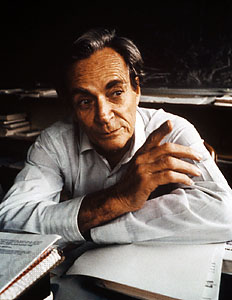
\includegraphics[scale=0.75]{feynman}
\end{center}
\end{document}